\chapter{Stand der Technik}\label{ch:background}

Zum Aufsetzen einer Hybrid Cloud Umgebung und dem Entwickeln einer auf dieser laufenden Anwendungen werden verschiedene Grundlagen benötigt. Grundwissen über die unterschiedlichen Speichertypen ist notwendig, um die Herausforderungen eines verteilten Speichersystems zu verstehen. Ebenfalls ist fundiertes Wissen über die Cloud, ihre Umsetzung und Typen wichtig, um in der Lage sein, effiziente Anwendungen für diese zu entwickeln.

In diesem Kapitel werden diese Hintergründe erläutert.

\section{Speicher Lösungen}
Speicherung von Daten ist ein wichtiges Thema in der IT, wodurch unzählige Technologien entstanden sind. Hier werden erst Hardware Speicher beschrieben und danach verschiedene Arten, diesen innerhalb von Rechnernetzwerken zusammenzustellen.

\begin{figure}[hbt]
	\centering
	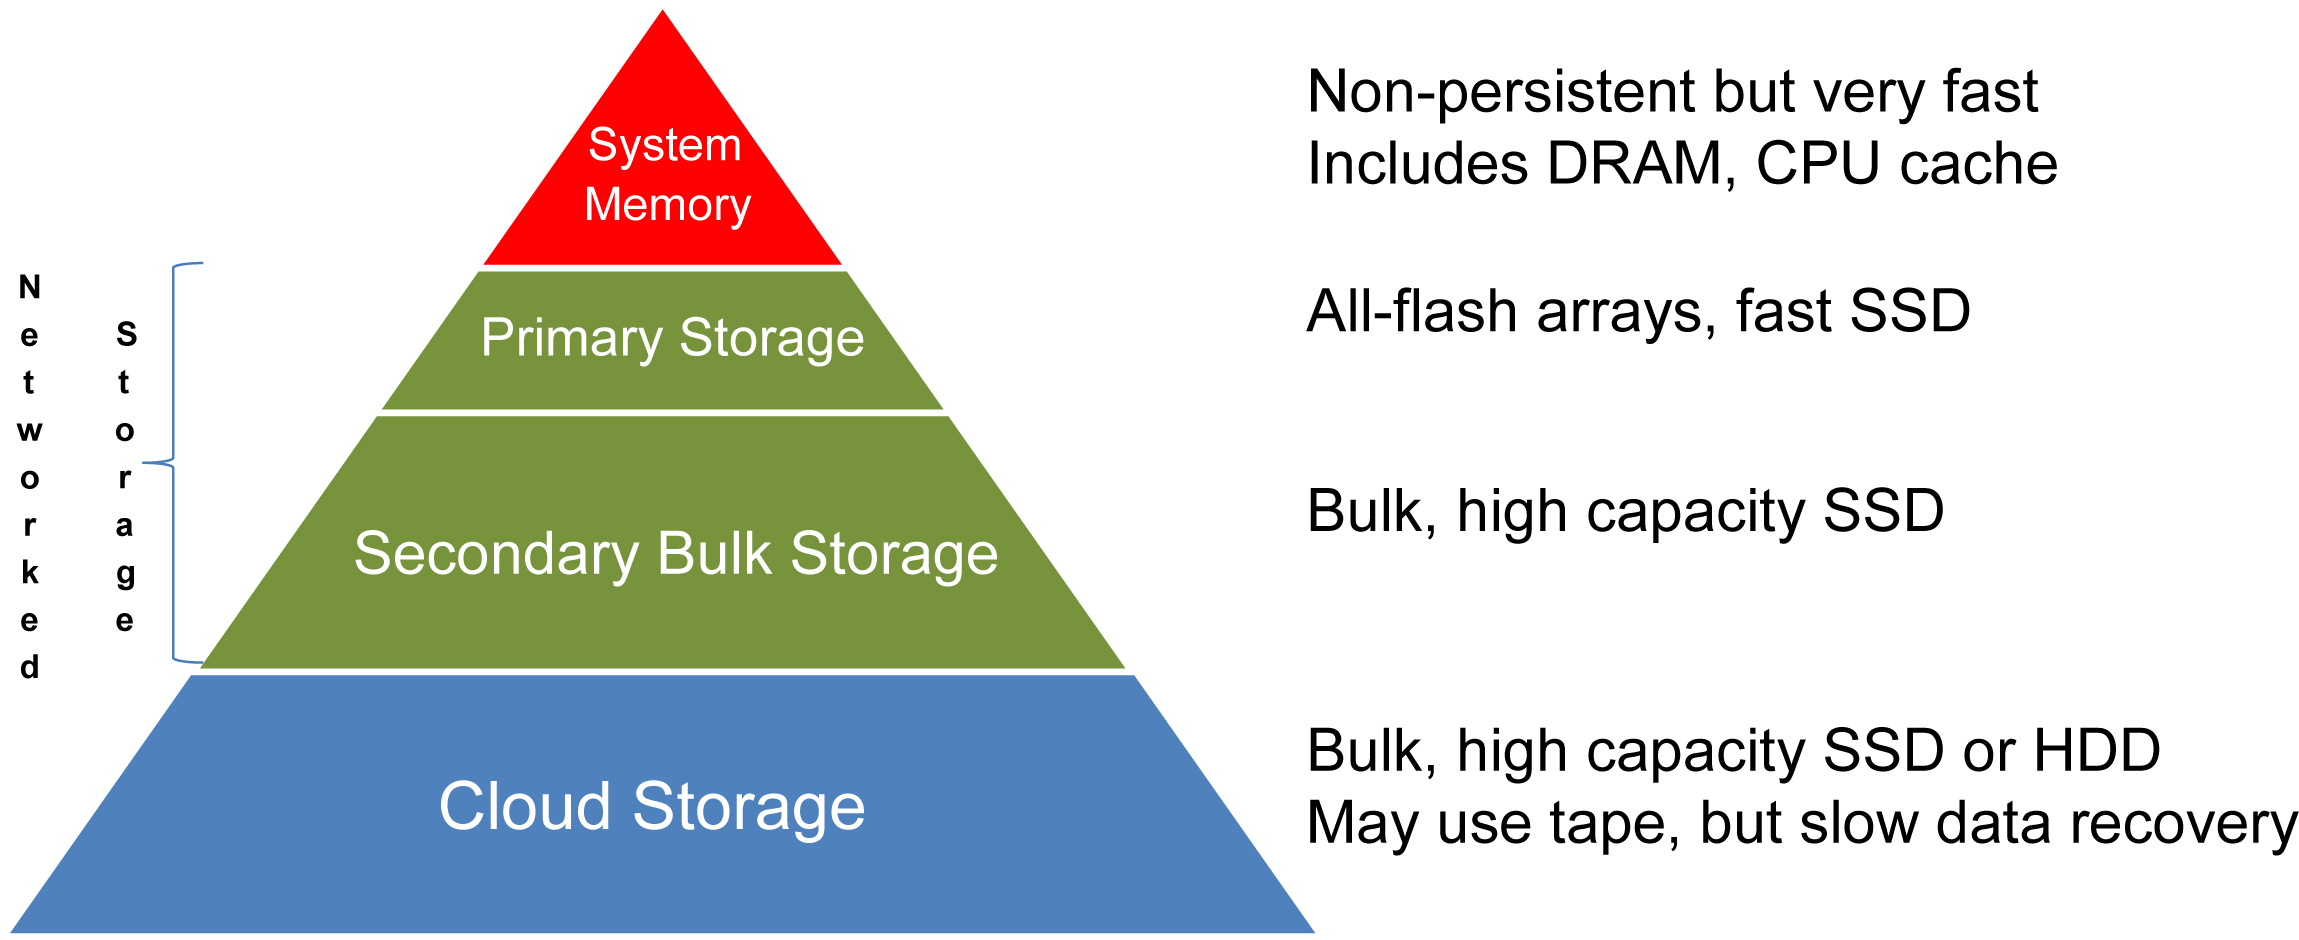
\includegraphics[scale=0.75]{images/storage-pyramide}
	\caption{Speicher Pyramide \parencite{kaufmann.2016}}
	\label{fig:storagepyramide}
\end{figure}

Prinzipiell kann Speicher immer in eine Art Hierarchie eingeteilt werden. Extrem häufige verwendete Daten landen auf der Ersten Ebene. Diese wird meistens in Form von Cache oder RAM bereitgestellt und bietet extrem kurze Latenz, aber nur geringen Speicherumfang.

Auf der nächsten Ebene stehen schnelle Speichermedien, zum Beispiel SSDs. Direkt darunter ordnen sich klassische Festplatten Speicher ein, die den Großteil des Speichervolumens zur Verfügung stellen. Sie haben höhere Latenzen sind aber dafür günstig und haben eine hohe Kapazität \parencite[Kap. 2, What is Computer Storage?]{kaufmann.2016}.

Mit der letzten Stufe ``Cloud Speicher'' wird sich intensiver in der \autoref{sec:cloud} auseinander gesetzt.

\subsection{Hardware}

Unabhängig von der Zusammenstellung umfänglicher Speicherlösungen, müssen die Daten trotzdem irgendwann auf einen Hardwarespeicher geschrieben werden. Folgender Abschnitt erläutert, die allgemeine Funktion und geht auf einige der häufigsten verwendeten Typen ein.

\subsubsection{Hard Disk Drive (HDD)}

Hierbei handelt es sich um einen nicht volatilen Speicher, der digital kodierten Inhalte auf der magnetischen Oberfläche einer Platte speichert. Traditionell gibt es zwei Protokolle: SAS im kommerziellen und SATA im privaten Sektor \parencite{wikibooks.2016}.

Ein oder mehrere Leseköpfe werden mithilfe von Armen und einem Servomotor über die Platte bewegt, um relevante Stellen auszulesen. Bei der Herstellung von HDDs werden Tracks in die Platte geschrieben, die jeweils ein Label und Blockinformationen besitzen. Durch sie ist es einfacher, den Lesekopf zu platzieren. Jeder dieser Tracks kann bis zu einigen MBs an Daten beinhalten. Durch die Blockbildung bei I/O-Operationen kann häufig nur ein einzelner Block (64-256) geschrieben werden, wodurch Festplatten unnötig langsam werden. Durch neue Technologie können IOs in eine Warteschlange eingereiht werden, sodass die Platte kontinuierlich lesen und schreiben kann. Trotzdem ist nur eine maximale Geschwindigkeit von ungefähr 300 \gls{IOPS} das Limit für Platten mit 10.000 RPM \parencite[Kap. 3]{kaufmann.2016}.

Jede Festplatte hat heutzutage einige private Sektoren, auf denen Reparaturinformationen und Reserveblöcke gespeichert sind. Fällt ein Block in der Festplatte aus (durch zum Beispiel physikalische Beschädigung), kann dieser fließend ersetzt werden, sodass keine Daten verloren gehen. Kurz vor dem Ausfall einer Platte steigt diese Anzahl der Lesefehler einer Platte massiv an, sodass eine Datenreovery versucht werden kann. Leider ist dies keine verlässliche Methode, um Daten zu sichern, sodass andere Methoden verwendet werden sollten \parencite[Kap. 3]{kaufmann.2016}.

Um Datenverlust durch Plattenausfälle entgegenzuwirken, besteht die Möglichkeit der Verwendung von so genannten RAIDs. Dies ist eine Methode, bei der mehrere HDDs so zusammengeschaltet werden, sodass bei dem Ausfall einer Einzelnen die Daten weiterhin verfügbar sind \parencite{wikibooks.2016}.

Festplatten sind gut erforscht, es treten extrem selten unbekannte Probleme auf und werden seit Jahrzehnten verwendet, ihr Speicher ist extrem günstig geworden und in Masse verfügbar. Ihr größter Nachteil ist eine sehr geringe I/O-Geschwindigkeit im Vergleich mit neueren Technologien \parencite[Kap. 3]{kaufmann.2016}.

\subsubsection{Solid State Drive (SSD)}

Im Jahr 2007 wurde der erste SSD-Speicher vermarktet und stach durch extrem hohe Zugriffszahlen heraus. Diese waren bei 4000 \gls{IOPS} bereits um das zehnfache höher als die klassischer Festplatten. Heutzutage ist es möglich IOPS Zahlen im Millionenbereich zu erreichen, was eine Revolution für Speicher bedeutet \parencite[Kap. 3]{kaufmann.2016}.

\begin{figure}[hbt]
	\centering
	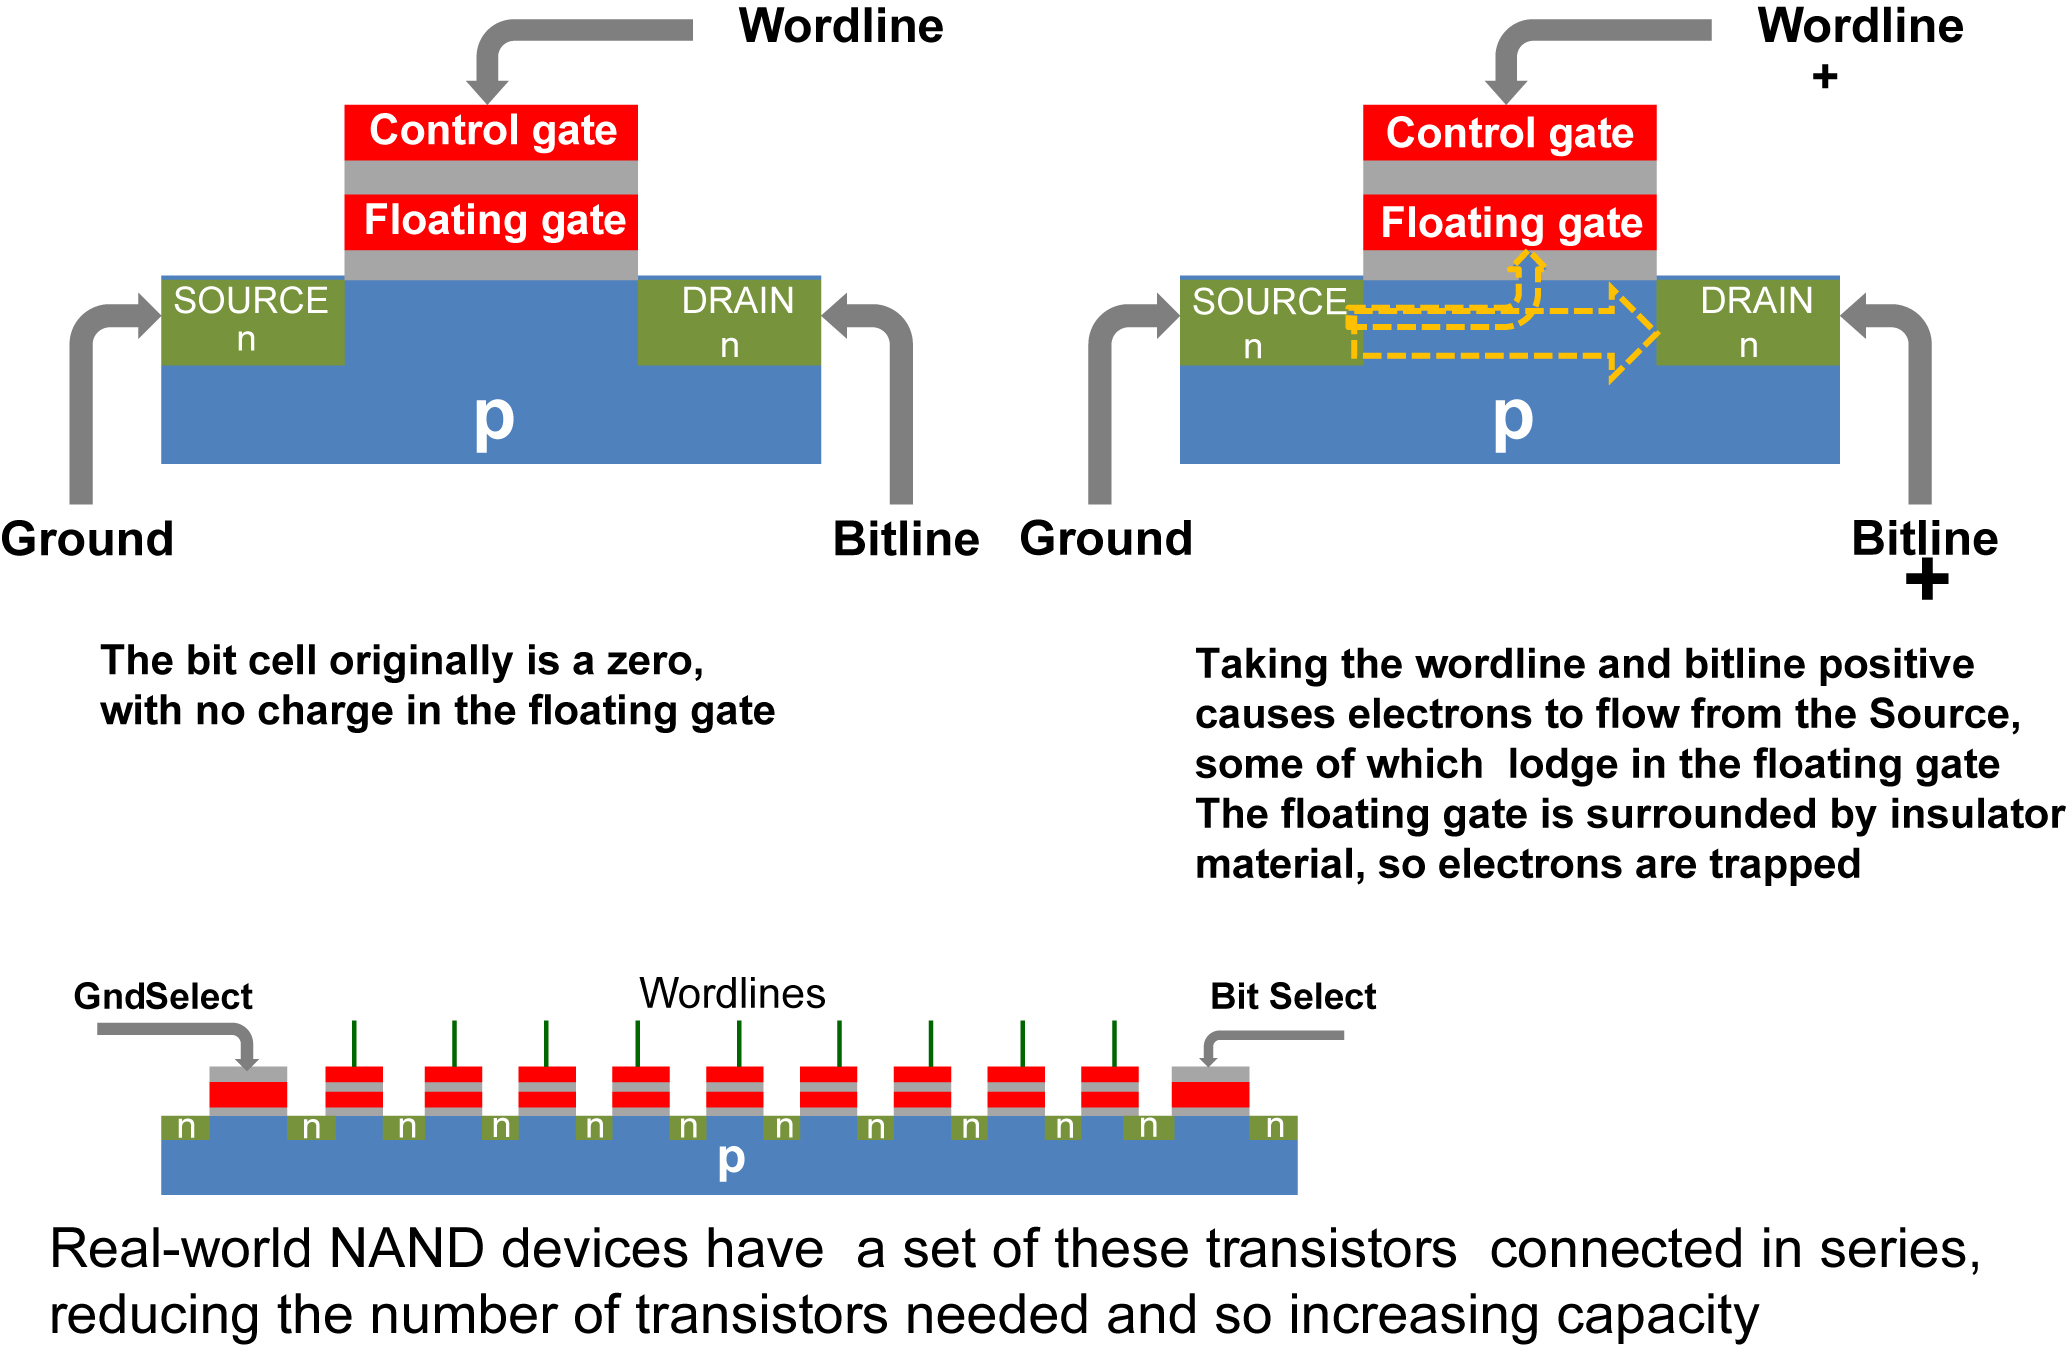
\includegraphics[scale=0.85]{images/flash}
	\caption{Funktionsweise eines NAND-Flashspeichers \parencite{kaufmann.2016}}
	\label{fig:flash}
\end{figure}

SSDs benutzen Nicht-Und (NAND) memory chips zum Speichern einzelner Bitinformationen. Von diesen Zellen gibt es dann einige Millionen, die beliebig adressiert werden können (Random Access Memory). Innerhalb eines so genannten Floating Gate können nun Elektronen eingefangen werden, um eine binäre Eins zu repräsentieren. Im Ausgangszustand sind diese ``Fallen'' leer, um einen Nullinformationen zu speichern. Sobald der Speichercontroller eine Zelle laden will, wird der Einlasstransistor geöffnet und einige Elektronen in der Zelle für eine beliebig lange Zeit gefangen.

Dieser Prozess findet in \autoref{fig:flash} statt, wenn auf der Bit- und Wordline eine positive Ladung gesetzt wird. Meistens liegen mehrere Zellen auf einer Reihe, was den Leseprozess verkomplizieren kann. Es wird eine niedrige Spannung an alle Wordlines angelegt, wodurch bei geladenen Zellen eine Konduktivität festgestellt werden kann. 

Wird eine einzelne Zelle zu häufig beschrieben, kann diese Isolation verlieren, wodurch sie unnutzbar zum Speichern wird. Schreibstrategien und Reservezellen werden verwendet, um dem vorzubeugen.	

Zum Löschen der Zellen wird eine hohe negative Spannung an die Zellen angelegt, wodurch die gefangenen Elektronen aus den Floating Gates heraus gestoßen werden. Dies passiert meistens in fest definierten Pages, sodass keine speziellen Blöcke gelöscht werden können. Nach dem Löschen eines Blockes wird dessen Zeiger auf eine vorher geleerte Page bewegt und der Block als ``discared'' markiert. Sind innerhalb einer Page genug Blöcke in diesem Zustand, werden die verbleibenden Daten verschoben und die gesamte Page gelöscht und Teil des freien Speichers der SSD \parencite{kaufmann.2016}. 
Durch diesen Prozess ist das Löschen von Dateien nicht mehr zuverlässig, da die Daten noch für lange Zeit innerhalb eines ``discared'' Blockes liegen können, der erst wesentlich später vom Controller gelöscht wird.

SSDs können über das SATA-Protokoll angeschlossen werden, aber in den letzten Jahren wurde das wesentlich performantere NVMe entwickelt.

Da dieser Speicher keine sich bewegenden Teile hat, ist er wesentlich robuster was Schläge, Vibrationen und hohe Temperaturen angeht. Ebenfalls ist der Strombedarf wesentlich geringer, was zusammen mit den vorherigen Punkten den Betrieb von SSDs in großen Rechenzentren wesentlich einfacher und günstiger macht.

Trotzdem gibt es auch einige Nachteile von Flashspeicheren: Die meisten Anwendungen sind nicht darauf ausgelegt, so hohe Zugriffszahlen zu unterstützen. In der Vergangenheit hat I/O immer ein Bottleneck in Applikationen dargestellt, sodass die meisten Programme entsprechend designed wurden.
Dies zieht sich durch die gesamte Softwarelandschaft und auch die geläufigen Betriebssysteme sind nicht in der Lage, diese neue Geschwindigkeit voll auszunutzen. Ebenfalls ist das SATA Interface nicht perfekt für SSDs, da es ursprünglich dafür designed war, die niedrigen Bandbreiten von Festplatten auszugleichen \parencite[Kap. 3]{kaufmann.2016}.


\subsubsection{Bandlaufwerk}

Bandlaufwerke funktionieren im Grunde wie die früher verwendeten Kassetten. Innerhalb des Laufwerkes befindet sich ein dünner Streifen aus Plastik mit einer magnetischen Oberfläche. Dieser wird, ähnlich wie bei Festplatten, mit digitalen Daten beschrieben. 

Es kann nicht auf beliebige Bereiche des Bandes zugegriffen werden, Lesen und Schreiben erfolgt immer sequentiell. Das Laufwerk muss von Anfang bis Ende durchlaufen werden, um I/O Aktionen durchführen zu können \parencite{adrc.2009}.

Ein Bandlaufwerk verwendet einen kleinen Motor, um das Band auf- und abzuwickeln. Dabei wandert dieses entlang eines Lese- und Schreibkopfes. Um Unterschiede zwischen der Geschwindigkeit der ankommenden Daten vom Computer und der begrenzten \gls{IOPS} des Laufwerkes auszugleichen, wird eine Steuereinheit verwendet. Diese regelt Fehlerhandling, Puffer und andere logische Operationen.

Informationen werden in die Steuereinheit geladen und dann auf das Band geschrieben. Dieser Prozess wiederholt sich solange, bis keine Daten mehr vorhanden sind.

Aufgrund von geringen Kosten und hoher Lebenszeit wird diese Art von Laufwerk immer noch häufig verwendet. Besonders of wird es für Backupszenarien genutzt, da hier die Nachteile des nur sequentiellen Zugriffes auf Daten keine große Rolle spielen \parencite{adrc.2009}. 

\subsection{Speicheranbindung über Netzwerke}
\subsubsection{Direct Attached Storage (DAS)}

Bei \ac{DAS} handelt es sich um externen Speicher, der direkt mit einem oder mehreren Servern über ein \gls{SCSI} Interface verbunden ist. Dabei wird kein Netzwerk verwendet. Es gibt verschiedene Typen von \ac{DAS}, bei manchen werden nur beliebige Platten zusammengewürfelt (\ac{JBOD}), bei anderen ganze Plattenarrays angeschlossen.
Hierbei handelt sich um den ältesten Speichertypen, der lange vor dem Entstehen von SAN oder NAS verwendet wurde.

Es kann nur eine begrenzte Anzahl von \ac{DAS} an einen Rechner angeschlossen werden, da die Anzahl von SCSI-Schnittstellen an Servern limitiert ist. Dadurch ist diese Art von Speicher leider nur begrenzt skalierbar.

Ein weiterer großer Nachteil von direkt angebundenen Speicher ist, dass bei einem Ausfall des Servers ein wesentlicher Teil der Daten nicht mehr erreichbar ist. Die Verfügbarkeit der Daten hängt also nicht nur vom Speicher selber ab, sondern auch von dem bereitstellenden Server.

Wird das Laufwerk an mehrere Server angeschlossen, um obige, Problem entgegenzuwirken, erhöht sich durch einen Ausfall die Zugriffszeit beträchtlich \parencite[Kap. 1, Disk Storage Systems]{gupta.2002}.

Der größte Vorteil von DAS Geräten ist, dass sie einfach aufzusetzen und zu warten sind, da keine Netzwerkkenntnisse oder Hardware benötigt werden. Dies bedeutet geringe Kosten und einfache Handhabung \parencite{beal.2017}.

\subsubsection{Network Attached Storage (NAS)}

\ac{NAS} ist ein einfaches System, um Daten an einer einheitlichen Stelle im Netzwerk zu speichern. Hierdurch werden die Daten von den Servern selber zu speziell zur Speicherung ausgelegten Hardware wegbewegt. 

Ein NAS-Gerät ist spezialisierte Hardware mit meist zugehöriger Management Software. In den meisten Fällen muss es nur mit dem Firmennetzwerk verbunden und eingeschaltet werden. Ebenfalls ist der Speicher plattformunabhängig und kann mithilfe verschiedener Protokolle von jedem Client verwendet werden. Einige Beispiele für diese sind: HTTP (Internetanfragen), FTP oder TCP/IP. Ebenfalls können Datenanfragen über NFS (für Linux) oder SMB (für Windows) getätigt werden \parencite[Kap. 1, NAS Devices]{gupta.2002}.

Bei einem Daten Request wird die Anfrage an das NAS Gerät weitergeleitet, das die notwendige Daten an den Server zurück sendet, welcher diese dem Client zur Verfügung stellt.

NAS besitzt einige Vorteile: Es gibt eine deutliche Leistungssteigerung bei den Anwendungsservern, da I/O Operationen komplett auf der dedizierten Hardware ausgeführt werden. NAS Devices besitzen eine wesentlich bessere Skalierbarkeit als \ac{DAS} Geräte, es können beliebig viele neue Netzwerkspeicher zu einem System hinzugefügt werden.

Ebenfalls ist die Fehleranfälligkeit wesentlich geringer, wenn ein Anwendungsserver abstürzt, bleibt der Zugriff auf den NAS im Netzwerk immer noch erhalten.

Management und Einsatz sind auch einfach gehalten, die Geräte konfigurieren sich zu großen Teilen selber und sind mit jedem System ansprechbar.

Trotz all dieser Vorteile gibt es, besonders in großen Netzwerken, auch einige Nachteile. Anfragen von Clients erzeugen eine große Menge Netzwerkverkehr, der viel Bandbreite beansprucht. Sobald viele Request gleichzeitig auftreten, kann es deswegen auch zu Performanceeinbrüchen kommen.

Durch die Zentralisierung des Speichers wird dieser auch einfacher anfälliger für bösartige Attacken, Netzwerk Verkehr kann abgefangen oder modifiziert werden \parencite[Kap. 1, Adv. and Disadv. of NAS Devices]{gupta.2002}.


\subsubsection{Storage Area Network (SAN)}
\ac{SAN} wurden entwickelt, um enorme Mengen an Daten zu verarbeiten. Sie werden nicht direkt in das Client- oder Servernetzwerk eingebunden, sondern bilden ein eigenes, das die verschiedenen Speicher miteinander verbindet. Dieses kann dann nur durch die SAN Server angesprochen werden. Dies führt zu einem sehr sicheren Setup, da die Geräte vor den Clients komplett verborgen sind \parencite[Kap. 1, SANs]{gupta.2002}.

Es gibt mehrere wichtige Bestandteile: Die oben erwähnten Server stellen den Zugriffspunkt für Applikationsserver im normalen Netzwerk. Innerhalb des Netzwerks kann es verschiedene Speichertypen geben (RAIDs, JOBDs, Disk Storage Systems, Bandlaufwerke).
Interfaces werden verwendet, um den Speicher mit den Server zu verbinden und sie damit zu externalisieren. Mithilfe von SAN Interconnects können entfernte Speicher ebenfalls eingebunden werden. Hubs und Router werden benutzt, um verschiedene Speicher zusammenzuschließen, wobei Router das Signal immer nur zu einem Gerät weiterleiten und es nicht broadcasten.
Außerdem gibt es noch eine ganze Reihe an weiteren Geräten, die für die Kommunikation zwischen verschiedenen Protokollen und Technologien verantwortlich sind \parencite[Kap. 2, SAN Components and Building Blocks]{gupta.2002}.

Ein vereinfachtes Setup kann in \autoref{fig:storageareanetwork} betrachtet werden.

\begin{figure}[hbt]
	\centering
	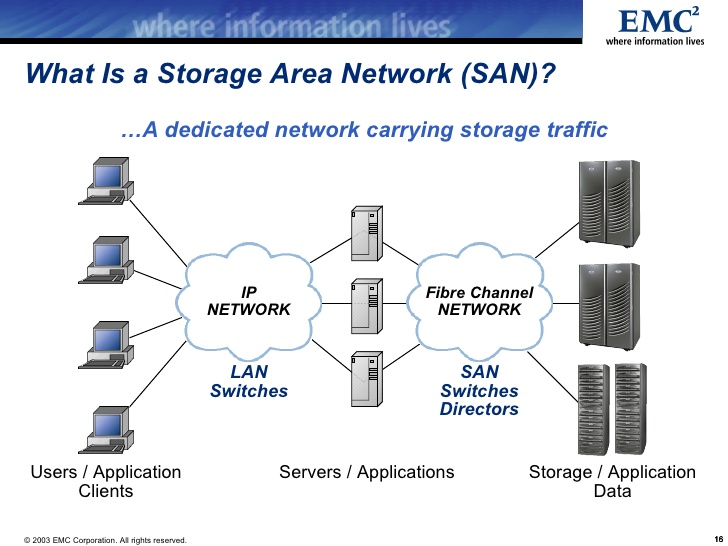
\includegraphics[scale=0.9]{images/storage-area-network}
	\caption{Typische SAN Konstruktion \parencite[Kap. 1]{gupta.2002}}
	\label{fig:storageareanetwork}
\end{figure}

Durch dieses eigene Netzwerke können einige Vorteile ausgenutzt werden, die so bei \ac{NAS} nicht oder nur schwer zu erreichen sind. Zur Verbindung der Geräte können Hochleistungsnetzwerke wie FibreChannel verwendet werden, die wesentlich performanter sind als Ethernet. Da das SAN getrennt vom Netzwerk der Applikationsserver ist, muss keine Bandbreite geteilt werden, was ebenfalls die Anwendungen schneller macht. Genauso wie bei NAS werden I/O-Aktionen auf die SAN-Geräte verlagert und es können zusätzlich Performance intensive Backups isoliert im SAN erledigt werden \parencite[Kap. 1, SANs]{gupta.2002}.

Das Filesystem von SANs wird nicht von den Geräten selber verwaltet, sondern von den entsprechenden Fileservern. SANs bieten einfachen Blockzugriff auf die Daten, für die Server sind sie nur weitere Festplatten. Dadurch ist es einfacher, das SAN beliebig zu skalieren, da einfach nur neue Speichergeräte hinzugefügt werden müssen. Die Ausfallsicherheit wird ebenfalls höher, da meistens verschiedene Server Zugriff auf das SAN haben und einfach ein weiterer angesprochen werden kann, falls ein Ausfall stattfindet.

Es gibt optimierte Software zur Verwaltung von SANs, die höhere Performance ermöglichen.

Ein großer Nachteil von SANs ist, dass sie sehr komplex aufzusetzen sind und auch die Kosten wesentlich höher sind als bei NAS Lösungen \parencite[Kap. 2]{gupta.2002}.

\section{Dateisysteme}

Für Anwendungen und Nutzer organisiert ein Dateisystem eine abstrahierte Sicht auf sämtlichen Daten. Es stellt eine Schnittstelle zur Verfügung für Online-, Offline- und Programmzugriff. Ein Filesystem besteht aus einer Sammlung aller Dateien und einer Ordnerstruktur, die erstere organisiert und beschreibt. 

Das Betriebssystem ordnet Speicherblöcke logischen Einheiten zu, so genannten \textbf{Files}. Die physikalischen Eigenschaften des Speichergerätes werden hiermit vor dem Nutzer verborgen. SSDs, HDDs, Online Speicher und sogar Cluster-Dateisysteme können hierdurch auf die gleiche Art betrachtet werden \parencite{silberschatz.2012}.

Im Folgenden werden verschieden Clustersysteme, ihre Vor- und Nachteile untersucht.

\subsection{IBM Spectrum Scale - GPFS}

Bei IBM Spectrum Scale handelt es sich um ein System, dass den gleichzeitigen Zugriff auf ein oder mehrere Dateisysteme zur Verfügung stellt von verschiedenen Knoten. Diesen können mithilfe von unterschiedlichsten Techniken den Zugriff zur Verfügung stellen (SAN, NAS, DAS) und ermöglichen das Aufsetzen von einem hochperformanten skalierbaren Netzwerkes \parencite[S. 1]{ibm.2017}.

Neben einfachen Datenzugriff werden ein Vielzahl von zusätzlichen Features geboten: Datei Duplizierung, Regel basiertes Speicher Management, Kommunikation und Zusammenschluss verschiedener Rechenzentren und diverse andere. Auf diese wird hier aber nur sehr grob eingegangen, da sie größtenteils unrelevant für die Arbeit sind und deren Umfang übersteigen würden.

\textbf{Hauptkomponenten und Funktionen}

Von jedem Knoten des Clusters kann gleichzeitig auf sämtliche Daten zugegriffen werden. Aufgrund der \gls{POSIX} Kompatibilität kann der Zugriff über Systemfunktionen (open, read, write) oder speziellen APIs erfolgen. Dies vereinfacht die Bedienung erheblich, da der Cluster für den einzelnen Rechner wie eine ``normale'' Festplatte erscheint. Auf jedem GPFS Knoten sind drei Hauptkomponenten installiert:

\begin{itemize}
	\item \textbf{GPFS Administration Kommandos} \\
	Eine Reihe von Skripts und Programme, die Konfigurationen ändern und Operationen auslösen können. Ausgeführte Kommandos können beliebige Knoten betreffen und werden entsprechend weitergeleitet und auf entfernten Systemen ausgeführt.
	\item \textbf{GPFS Kernel Erweiterung} \\
	Diese Erweiterung bietet ein Interface zum Betriebssystem und ermöglicht es GPFS als natives Dateisystem zu registrieren. Hierdurch erscheint der gesamte Cluster für eine Applikation wie eine einzelne Festplatte. Der Kernel führte diese entweder lokal auf verfügbarem Speicher aus oder leitet sie mithilfe des GPFS Daemon zu anderen Geräten weiter.
	\item \textbf{GPFS Daemon} \\
	Aufgabe dieses multithreaded Programmes ist das Ausführen sämtlicher Schreib-, Lese- und Pufferaktionen. Er sorgt auch für die Datenkonsistenz des Gesamtsystems. Zusätzlich zu den I/O Aktionen wird auch die Kommunikation mit anderen Knoten im System ausgeführt, um Konfigurationsänderungen, Wiederherstellung und parallele Updates durchzuführen.
	Ebenfalls enthalten ist die Network Shared Disk Komponente, die Cluster weite Benennung von und den Zugriff auf Speicher zur Verfügung stellt \parencite[S. 6]{ibm.2017}.  
\end{itemize} 

\textbf{Cluster Arten}

Es kann eine Vielzahl von Cluster Konfigurationen erreicht werden, da Spectrum Scale unterschiedlichste Betriebssysteme unterstützt (speziell Linux, AIX, Windows) und Speicher auf verschiedene Arten anschließbar ist. Im Folgenden werden zwei häufige Szenarien vorgestellt.

Eine Variante ist der Anschluss von sämtlichen Knoten an das selbe Storage Area Network. Ist dies nicht der Fall, können nur einzelne Nodes angeschlossen sein als \ac{NSD} Server und die verbleibenden sind \ac{NSD} Klienten. Hierbei wird eine klassische Server-Client Architektur aufsetzen bei der eine Vielzahl von GPFS Klienten auf eine kleinere Anzahl von GPFS Servern mit Speicheranbindung zugreift \parencite[S. 8]{ibm.2017}.

\begin{figure}[hbt]
	\centering
	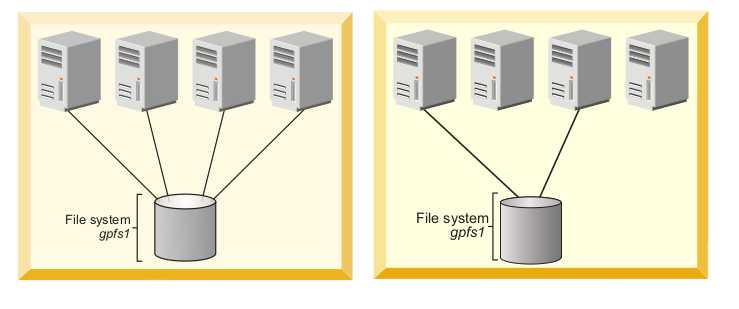
\includegraphics[scale=0.6]{images/gpfs-architectures}
	\caption{Anbindung an alle Knoten (links) und Server-Klient Architektur (rechts) \parencite[S. 8]{ibm.2017}}
	\label{fig:gpfsarchitecture}
\end{figure}

\textbf{Verbindung mit Cloud Diensten}

Cloud Dienste mit Spectrum Scale bieten zwei Funktionsweisen: \textbf{Cloud Tiering} und \textbf{Data Sharing}. Es können maximal vier verschiedene Knoten und ein Dateisystem für diese Dienste verwendet werden \parencite{mani.2017}.

Im ersten Szenario werden so genannte kalte Daten (also Dateien, die selten benutzt werden und geringe Zugriffszahlen haben) in der Cloud gespeichert, um die schnellen lokalen Datenspeicher zu entlasten. Dadurch kann die Clusterperformance erhöht und kosten für zusätzlichen Speicher gespart werden. Diese Funktion ist das Information Lifecycle Management (\ac{ILM}) System eingebunden und ermöglicht es den Administratoren Strategien zu definieren, um die Auslagerung bei bestimmten Daten auszulösen.
Es sollten nur kalte Files in der Cloud gespeichert werden, da diese bei Zugriff zu downloaden sind, was die Latenz massiv erhöht \parencite[S. 107]{ibm.2017}.
Lokal wird ein Cloud Verzeichnis angelegt, welches alle migrierten Daten auflistet. Wird auf einen Datei-Stub zugegriffen, kann die ferne Information heruntergeladen werden. In der Cloud liegen pro File zwei verschlüsselte Dateien, eins für die eigentlichen Daten und ein zweites mit Metadaten (Besitzer, Zugriff, ...) \parencite[S. 108]{ibm.2017}.

Beim Cloud Sharing ermöglicht das Teilen von lokalen Daten mit verschiedenen Arten von Objekt Speichern (\autoref{subsec:objectstorage}). Dieser Export kann ebenfalls durch IML Strategien in regelmäßigen Zyklen ausgelöst werden, um zum Beispiel Daten in der Cloud aktuell zu halten. Diese können dann von anderen Applikationen verwendet werden. Es ist ebenfalls ein Import von Object Storage System möglich, um die lokalen Daten ggf. zu erweitern.
Der Export wird parallel mit allen Cloud Dienst Knoten durchgeführt. Dabei kann eine Liste aller Daten in einem Manifest gespeichert werden, um diese später nachzuverfolgen.
Der größte Unterschied zur Migration beim Cloud Tiering ist, dass die Dateien in der Cloud nicht verschlüsselt werden, da sie auch für andere Nutzer verfügbar sein sollen und dass nach einem Transfer keine Verbindung (keine Updates bei späteren Änderungen) mehr zwischen lokalen und entfernten Files besteht \parencite[S. 109]{ibm.2017}.

Konfiguration dieser beiden Funktionalitäten kann mit dem \lstinline|mmcloudgateway| Programm vorgenommen werden \parencite{ibmadmin.2017}.

\subsection{Apache Hadoop - HDFS}

Apache Hadoop (ab hier nur noch Hadoop) ist ein Framework zu Entwicklung von massiven verteilten Systemen. Es ist in der Lage große Mengen von Daten, sowohl strukturiert wie auch unstrukturiert, über viele verteilte Berechnungsknoten zu verteilen und zu bearbeiten. Das Hauptsystem von Hadoop verwendet ein eigenes Dateisystem HDFS \parencite[Kap. I,1]{alapati.2016}.

Diese System sorgt für eine automatische Datenreplikation und unterstützt ebenfalls das leichte Hinzufügen von weiteren Servern mit zusätzlichen Diskstorage. Ein typischer Hadoop Cluster besteht aus Master- (hier läuft die Hadoop Software), Arbeiterknoten (Bereitstellung von Speicher mit HDFS und Rechenleistung mit \ac{YARN}) und so genannten Edge Servern (Zugriff auf den Cluster zum Ausführen von Programmen). Zusätzlich kann es noch Server für zusätzliche Frameworks geben und Datenbanken für spezielle Metadaten \parencite[Kap. I,1]{alapati.2016}.

Bearbeitung der Daten kann mithilfe verschiedener Anwendungsframeworks passieren, besonders beliebt ist hierbei MapReduce und Apache Spark.

Standardmäßig repliziert HDFS jeden Datensatz dreimal, um eine hohe Ausfalltoleranz zu garantieren. Es wird ein  write-once-read-many (\ac{WORM}) Zugriffsmodel verwendet, sodass Konsistenz kein Problem darstellt, da immer nur ein Nutzer auf eine Datei schreiben kann. Daten werden in große Blöcke (zum Beispiel 256 MB) aufgeteilt und auf verschiedenen Maschinen gespeichert. Hierdurch können auch sehr große Files gesichert werden, die für einzelne Maschinen zu viel Speicher verbrauchen würden. Metdaten für alle Blöcke werden innerhalb einer NameNode im RAM und auf konsistenten Speicher gespeichert  \parencite[Kap. I,2]{alapati.2016}.

Hadoop kann auch komplett in der Cloud verwendet werden, es gibt einige Hosting Anbieter (Amazon EC2, Google Computing Engine), die einen dynamischen Funktionsumfang zur Verfügung stellen \parencite[Kap. I, 1]{alapati.2016}.

\subsection{Google File System - GFS} \todo{Really wanna do that?}
\subsection{Objekt Dateisysteme} \label{subsec:objectstorage}

Objekt Speicher ist eine moderne Speicher Technologie und eine logische Weiterentwicklung von Block- oder Dateispeicher. Es soll Probleme von klassischen Lösungen wie komplexe Speicherhierachie, Defragmentierung von File Systemen, sowie Sicherheit und Zugriff umgehen.

\begin{figure}[hbt]
	\centering
	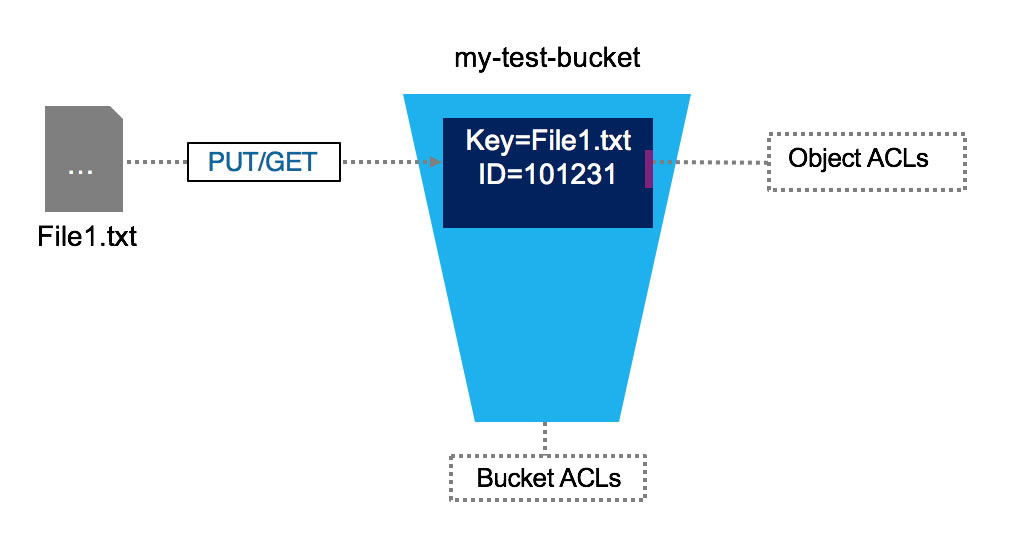
\includegraphics[scale=0.4]{images/object-storage}
	\caption{Komponenten von Objekt Speichern \parencite[S. 5]{Rios.2017}}
	\label{fig:objectstorage}
\end{figure}

Dieser Typ von Dateisystem umfasst drei Hauptkomponente:

\begin{itemize}
	\item \textbf{Daten:}\\
	 Nutzer und Anwendungsinformationen, die persistent hinterlegt werden müssen. Jede Art von Format ist hierbei unterstützt.
	\item \textbf{Metadaten:}\\
	 Diese sind Informationen über die eigentlichen Daten. Beispiele hierfür sind Dateigröße oder Uploadzeit. Ebenfalls können benutzerdefiniert Schlüssel-Wert Paare von nutzenden Anwendungen gespeichert werden. Diese sind von den Applikationen oder Usern zu jeder Zeit frei veränderbar. Eine Besonderheit dieses File Systems ist, dass die Metadaten zusammen mit den eigentlichen Daten gespeichert werden.
	\item \textbf{\ac{UUID}:} Diese eindeutige ID wird jedem Objekt im Speicher zugeordnet. Mit ihr können Daten unterschieden  und gefunden werden, unabhängig von der physikalischen Position der eigentlichen Informationen.
\end{itemize}

Durch obige Eigenschaften wird eine flache Hierarchie erzeugt, die Probleme mit außer Kontrolle geratenen Metadaten Speichern verhindert. Daten können in sogenannten Buckets zusammengefasst werden, um eine logische Strukturierung einzuführen und ebenfalls die Zugriffsrechte von Nutzern einschränken können.  

Da diese Art von Daten fast immer in der Cloud oder auf einem entfernen Server verwendet wird, bieten sich besonders REST Schnittstellen zum Zugriff auf die Daten an \parencite[S. 4f]{Rios.2017}.

\todo{Validate Information for other systems}


\section{Cloud Computing}\label{sec:cloud}
%Insert General explanation here
\todo{Weitere Quellen benutzen}

Cloud Computing kann als eine neue Art der Bereitstellung von Programmen, Diensten und Infrastruktur betrachtet werden, die häufig virtualisiert und automatisch skalierbar ist. Es ist die logische Weiterentwicklung von Netzwerk oder Internet Computing und hilft dabei vorhandene Ressourcen besser auszunutzen. 
Software, Laufzeiten und sogar Plattformen werden in einem verteilten Serverclusters angeboten. Diese können dann von jeder Art  Client Geräten (Personal Computer, Smartphones, \ac{IoT} Devices) angesprochen werden. Außer Anwendungen werden häufig  auch Speicher, bestimmte Dienste oder Entwicklungswerkzeuge über die Cloud angeboten \parencite[S. 3]{furth.2010}.

Ein großer Vorteil von Cloud Umgebung ist die Dezentralisierung von Anwendungen. Statt für eine Applikation einen einzelnen Server zu nutzen, wird diese in einem Netz von diesen virtualisiert. Dieses Netz von Servern kann eine Vielzahl von Anwendungen provisonieren und bei Bedarf automatisch höhere Leistung zuordnen. Hierdurch werden Kosten gespart und eine bessere Verfügbarkeit garantiert \parencite[S. 7]{furth.2010}.

Es gibt einige Schlüsseltechnologien die Cloud Computing erst ermöglichen. 

Zum einen ist Virtualisierung extrem wichtig, da Container und virtuelle Maschinen auf verschiedenen Servern gehostet werden können (Entkopplung von Anwendung, OS, Hardware und Nutzerdaten), um unterschiedliche Anwendungen für globale Zugriffspunkte bereitzustellen. 
Sobald mehr Performance notwendig ist (mehr Zugriffe) können diesen mehr Serverleistung bekommen oder es werden weitere Instanzen auf zusätzlichen Rechnern erzeugt.
Um diese effektiv umzusetzen besitzen Cloud Systeme einen Load Balancer, der automatisch Zugriffe auf die bereitstellenden Server verteilt und dafür sorgt, dass zum Beispiel Sitzungen aufrecht erhalten werden (Die Zugriffe eines Nutzer landen immer auf dem selben Server).
Zur Loslösung von Speicher wird dieser gerne in separaten \acs{SAN} ausgelagert \parencite[S. 22]{rafaels.2015}.
\subsection{Cloud Modelle}
%On/Off Premise
%SaaS / PaaS / IaaS

Es gibt verschiedene Cloud Modelle, die jeweils unterschiedliche Features für den User bereitstellen. Hauptsächlich unterscheidet man hier zwischen \ac{IaaS}, \ac{PaaS} und \ac{SaaS}, welche aber auch gleichzeitig vom selben Anbieter zur Verfügung stehen können.

\begin{itemize}
	\item \textbf{IaaS}:\\
	Dem Nutzer hat die Kontrolle über das zu verwendende OS, den Speicher und gehostete Anwendungen. Nur die unterliegende Cloud Infrastruktur ist nicht veränderbar und häufig sind auch nur bestimmte Teile der Firewall anpassbar.
	\item \textbf{PaaS}:\\
	In diesem Fall hat der Nutzer keine Wahl was Betriebssystem, Netzwerk Fähigkeiten oder Speicher angeht, es existiert eine vorinstallierte Umgebung (Datenbanken, Frameworks, Laufzeiten, usw.) zum Ausführen von eigenen Applikationen. Begrenzt bestehen Konfigurationsmöglichkeiten für die Hosting Umgebung der Software. 
	\item \textbf{SaaS}:\\
	Es wird nur eine bestimmte Anwendung oder Interface dem Nutzer offengelegt. Er kann diese verwenden und ggf. seine persönliche Instanz konfigurieren, hat aber keinerlei Kontrolle über die unterliegend Laufzeit Umgebungen, den Speicher, das Netzwerk oder das OS \parencite[S. 15f]{rafaels.2015}.
\end{itemize}

Des weiteren können Cloud Server in verschiedenen Umgebungen installiert werden, um Zugriff, Sicherheit und Verfügbarkeit zu regulieren.

\begin{itemize}
	\item \textbf{Public Cloud}:\\
	Die Cloud Server sind öffentlich zugänglich und jeder kann Anwendungen erstellen und über die Infrastruktur bereitstellen. Das System wird meistens von einer Firma oder Regierungsstelle betrieben und die notwendige Hardware steht auf dessen Gelände. 
	\item \textbf{Private Cloud}:\\
	Die gesamte Cloud Infrastruktur wird nur für einen Kunden zur Verfügung gestellt und ist nur für diesen zugänglich. Sie kann von ihm oder einer dritten Gruppen gemanagt werden. Es besteht die Möglichkeit das System auf dem Gelände des Käufers zu installieren, um zum Beispiel Datensicherheit von kritischen Informationen zu gewährleisten. 
	\item \textbf{Hybrid Cloud}:\\
	Eine Hybrid Cloud verbindet Elemente aus einem öffentlichen und privaten Setup. Zum Beispiel können Teile der Berechnung in der public Cloud stattfinden und Personaldaten auf den privaten Servern verbleiben. Hierdurch können Datenschutz Bedenken berücksichtigt und die Vorteile öffentlichen Cloud Computings ausgenutzt werden. Zur Kommunikation zwischen den beiden Server Clustern können verschiedene standardisierte Schnittstellen verwendet werden (z.B. REST)  \parencite{rafaels.2015}.
\end{itemize}

\subsection{Anbieter}
Durch die Popularität von Cloud Computing gibt es mittlerweile an Vielzahl von Anbietern, an dieser Stelle werden nur die drei Größten (1. Amazon Web Services, 2. Microsoft, 3. IBM) kurz vorgestellt \parencite{statistia.2016}. Es wird sich hierbei auf Anbieter beschränkt, die mindestens \acs{PaaS} Funktionalitäten bieten, da für das Projekt dieser Arbeit eigene Anwendungen entwickelt werden müssen.


\textbf{Amazon Web Services}\\
Amazon ist im Moment der Marktführer mit fast 30 Prozent Marktanteil. Dies basiert zum einen darauf, dass \ac{AWS} er mit einer der ersten modernen Anbieter (seit 2002 in einfacher Form und seit 2006 mit den ersten Cloud Services) ist und es eine Vielzahl von Diensten gibt. Es gibt sowohl direkt ansprechbare Services für Speicher, Rechenleistung und Netzwerk Fähigkeiten für \acs{PaaS} Aufgaben als auch VM Systeme und Container für frei konfigurierbare Anwendungen (\acs{IaaS}).

Zum Beispiel die \ac{S3} Schnittstelle wurde von Amazon entwickelt und wird an einer Vielzahl von Stellen für die Kommunikation mit Objekt Speichersystemen verwendet \parencite{aws.2017}.

Aufgrund Amazons langer Geschichte mit Cloud Computing bieten sie im Moment die meisten Datencenter weltweit an und haben mehr Rechenleistung als die beiden anderen Konkurrenten zusammen. Auch bei der Auswahl von Diensten, haben Entwickler hier die meiste Vielfalt. Als Nachteil gelten eine gewisse Komplexität bei der Nutzung und eine Vernachlässigung des Hybrid und Privat Cloud Angebots \parencite{computerworlduk.2016}.


\textbf{Microsoft Azure}\\
Azure ist die Anwendungsplattform von Microsoft für eine öffentliche Cloud mit \acs{PaaS} und \acs{IaaS} Features. Sie ist spezialisiert für die Kombination mit Microsoft Diensten, Programmiersprachen und Lösungen. Mithilfe eines Management Portals lassen sich gehostete Applikationen verwalten. 

Es besteht die Möglichkeit \ac{VM}s oder Web Applikationen, für die eine Bandbreite an verschiedenen Diensten zur Verfügung steht, zu erzeugen. Es können ganze \acs{VM}s, Container oder auch nur einzelne lokale Komponenten (z.B. Speicher )aus on-premise Datencentern leicht in die Cloud gehoben werden.

Insgesamt gibt es viele Überschneidungen mit \acs{AWS}, aber die Kompatibilität mit Microsoft/Windows Komponenten ist wesentlich höher und andere Lösungen sind weniger vertreten \parencite{microsoft.2015}.


\textbf{IBM Bluemix}\\
Bei Bluemix handelt es sich um die \acs{PaaS}/\acs{IaaS} (wobei diese Funktion von Softlayer zur Verfügung gestellt werden) Lösung von IBM, die zuerst 2014 das erste Mal vorgestellt wurde. Außer der Möglichkeit \acs{VM}s, Root Server und Docker Container zu hosten, werden eine Vielzahl von IBM und Drittpartei Dienste angeboten, die von Speicher bis zu \acs{IoT} oder Maschinen Lernen reichen.

Es kann in einer Vielzahl populärer Sprache entwickelt werden (Node, PHP, Ruby, Java, Go...) und es gibt so genannte Buildpacks, die nicht vorhandene Laufzeit Umgebungen zum Teil nachrüsten. Ebenfalls kann Bluemix als private Cloud oder in einem "dedizierten" Modus zur Verfügung gestellt werden. Bei diesem wird garantiert, dass eine \acs{VM} nur auf einem isolierten Bare-Metal Server läuft.

In der Bluemix Konsole (Management Oberfläche) lassen sich auch einige \gls{DevOps} Funktionen konfigurieren. Es gibt einen eigenen Code Editor, Gitlab Integration und eine Buildpipeline für \ac{CI} \parencite{fassnacht.2016}.

Im Vergleich zur Konkurrenz bietet IBM viele \acs{IaaS} Dienste, kann aber bei Funktionen für Entwickler von Anwendungen nicht mithalten \parencite{computerwoche.2016}. 

\subsection{Entwicklung in einem Cloud System} \todo{Maybe remove or move to chapter 3}